% 附录

\appendix
% \appendixtitleformat  % 切换附录标题格式
\ctexset{
  chapter = {
    name = {附录},         % 设置章节名前缀为“附录”
    number = \Alph{chapter} % 使用 A, B, C 编号
  }
}
% \ctexset{chapter={
%   format={\centering \heiti \zihao{-2}}, 
%   number={   % 各章标题 黑体小2号 // 修改:标题和数字字号一致 
%     \arabic{chapter}},
%   name={,},
%   afterskip={0.5ex},
%   beforeskip={0.5ex}} % 标题之前的垂直间距
% }

\chapter{古诗评分体系}

% \renewcommand{\arraystretch}{1.2}  % 行距
\begin{longtable}{
    |>{\centering\arraybackslash}m{1.6cm} % 第一列,居中
    |>{\centering\arraybackslash}m{1cm}   % 第二列,居中
    |>{\centering\arraybackslash}m{1.6cm} % 第三列,居中
    |>{\centering\arraybackslash}m{1cm}   % 第四列,居中
    |>{\centering\arraybackslash}m{6cm}| % 第五列,居中
}
\caption{古诗评分体系} \label{tab:poem_scoring}\\
\hline
\textbf{维度} & \textbf{分值} & \textbf{子维度} & \textbf{小分} & \textbf{备注} \\
\hline
\endhead

\hline
\multicolumn{5}{|r|}{\small\sl 转下一页} \\
\hline
\endfoot

\endlastfoot

\multirow{12}{*}{\centering 格律规范} & 
\multirow{12}{*}{\centering 25} & 

    \multirow{4}{*}{\centering 平仄音韵} & 
    \multirow{4}{*}{\centering 10} & 
    \parbox[t]{6cm}{9-10:完全符合唐体格律(例:杜甫《登高》"风急天高猿啸哀,渚清沙白鸟飞回"平仄严谨)} \\ \cline{5-5}
    & & & & \parbox[t]{6cm}{7-8:个别拗句但有救(例:王维《终南别业》"行到水穷处"第三字拗,第四字救)} \\ \cline{5-5}
    & & & & \parbox[t]{6cm}{5-6:三平尾/三仄尾不超过两处(例:韦应物《滁州西涧》"独怜幽草涧边生"三平尾)} \\ \cline{5-5}
    & & & & \parbox[t]{6cm}{0-4:严重失律(例:打油诗体)} \\ \cline{3-5}

    & & 
    \multirow{4}{*}{\centering 对仗工稳} & 
    \multirow{4}{*}{\centering 10} & 
    \parbox[t]{6cm}{9-10:工对+借对精妙(例:李商隐《锦瑟》"庄生晓梦迷蝴蝶,望帝春心托杜鹃")} \\ \cline{5-5}
    & & & & \parbox[t]{6cm}{7-8:宽对但结构平衡(例:王勃《送杜少府》"海内存知己,天涯若比邻")} \\ \cline{5-5}
    & & & & \parbox[t]{6cm}{5-6:词性不对应(例:拙劣仿作"青山对绿水,饮酒对弹琴"名词对动词)} \\ \cline{5-5}
    & & & & \parbox[t]{6cm}{0-4:无对仗意识} \\ \cline{3-5}

    & & 
    \multirow{4}{*}{\centering 押韵协调} & 
    \multirow{4}{*}{\centering 5} & 
    \parbox[t]{6cm}{5:严格遵循平水韵(例:李白《静夜思》"床前明月光"押下平七阳韵)} \\ \cline{5-5}
    & & & & \parbox[t]{6cm}{3-4:邻韵通押(例:杜牧《清明》"纷"属文韵,"魂"属元韵通押)} \\ \cline{5-5}
    & & & & \parbox[t]{6cm}{1-2:出韵超过两处} \\ \cline{5-5}
    & & & & \parbox[t]{6cm}{0:完全无押韵} \\ \cline{1-5}

\multirow{8}{*}{\centering 意象意境} & 
\multirow{8}{*}{\centering 30} & 

    \multirow{4}{*}{\centering 古典运用} & 
    \multirow{4}{*}{\centering 20} & 
    \parbox[t]{6cm}{18-20:传统意象出新境(例:王维《使至塞上》"大漠孤烟直"重构"孤烟"意象)} \\ \cline{5-5}
    & & & & \parbox[t]{6cm}{14-17:精准使用经典意象(例:柳宗元《江雪》"孤舟蓑笠翁"的渔父符号)} \\ \cline{5-5}
    & & & & \parbox[t]{6cm}{10-13:意象堆砌无深意(例:劣作"残阳古道瘦马,西风落叶昏鸦")} \\ \cline{5-5}
    & & & & \parbox[t]{6cm}{0-9:意象误用(例:用"东篱"指代监狱)} \\ \cline{3-5}

    & & 
    \multirow{4}{*}{\centering 意境层次} & 
    \multirow{4}{*}{\centering 10} & 
    \parbox[t]{6cm}{9-10:多层意境交织(例:李商隐《夜雨寄北》时空折叠技法)} \\ \cline{5-5}
    & & & & \parbox[t]{6cm}{7-8:单一意境完整(例:孟浩然《春晓》的晨醒意境)} \\ \cline{5-5}
    & & & & \parbox[t]{6cm}{5-6:意境破碎(例:拼贴"明月松间照,股票涨停板")} \\ \cline{5-5}
    & & & & \parbox[t]{6cm}{0-4:无意境构建} \\ \cline{1-5}

\multirow{8}{*}{\centering 主题思想} & 
\multirow{8}{*}{\centering 20} & 

    \multirow{4}{*}{\centering 情感真挚} & 
    \multirow{4}{*}{\centering 12} & 
    \parbox[t]{6cm}{11-12:情志合一(例:杜甫《月夜》"遥怜小儿女,未解忆长安"的家国之痛)} \\ \cline{5-5}
    & & & & \parbox[t]{6cm}{9-10:情感明确但稍显直露(例:高适《别董大》"莫愁前路无知己")} \\ \cline{5-5}
    & & & & \parbox[t]{6cm}{6-8:情感造作(例:伪古风"朕与将军解战袍")} \\ \cline{5-5}
    & & & & \parbox[t]{6cm}{0-5:情感空洞} \\ \cline{3-5}

    & & 
    \multirow{4}{*}{\centering 思想传承} & 
    \multirow{4}{*}{\centering 8} & 
    \parbox[t]{6cm}{7-8:接通传统文脉(例:苏轼《题西林壁》对禅理的化用)} \\ \cline{5-5}
    & & & & \parbox[t]{6cm}{5-6:简单模仿前人(例:仿写"采菊东篱下"无新解)} \\ \cline{5-5}
    & & & & \parbox[t]{6cm}{3-4:曲解经典(例:将"仁者乐山"解为爱好登山)} \\ \cline{5-5}
    & & & & \parbox[t]{6cm}{0-2:思想谬误} \\ \cline{1-5}
    
\multirow{6}{*}{\centering 语言锤炼} & 
\multirow{6}{*}{\centering 15} & 

    \multirow{3}{*}{\centering 凝练度} & 
    \multirow{3}{*}{\centering 8} & 
    \parbox[t]{6cm}{7-8:字字珠玑(例:贾岛《题李凝幽居》"鸟宿池边树,僧敲月下门")} \\ \cline{5-5}
    & & & & \parbox[t]{6cm}{4-6:可删减1-2字(例:初稿"推"改为"敲"的炼字过程)} \\ \cline{5-5}
    & & & & \parbox[t]{6cm}{1-3:冗余明显(例:劣作"我看到青山高又高,绿水长流流不停")} \\ \cline{3-5}

    & & 
    \multirow{3}{*}{\centering 典雅度} & 
    \multirow{3}{*}{\centering 7} & 
    \parbox[t]{6cm}{6-7:文白交融自然(例:李清照《声声慢》"寻寻觅觅"的白话感)} \\ \cline{5-5}
    & & & & \parbox[t]{6cm}{4-5:文言生硬(例:强行用"之乎者也"凑韵)} \\ \cline{5-5}
    & & & & \parbox[t]{6cm}{1-3:语体混乱(例:夹杂"OK""Hi"等外来词)} \\ \cline{1-5}
        
\multirow{4}{*}{\centering 创新性} & 
\multirow{4}{*}{\centering 10} & 

    \multirow{4}{*}{\centering \textbackslash} & 
    \multirow{4}{*}{\centering \textbackslash} & 
    \parbox[t]{6cm}{9-10:传统技法新用(例:王安石《泊船瓜洲》"绿"字形容词动用)} \\ \cline{5-5}
    & & & & \parbox[t]{6cm}{7-8:有限度创新(例:崔颢《黄鹤楼》前半打破律诗常规)} \\ \cline{5-5}
    & & & & \parbox[t]{6cm}{5-6:为变而变(例:强行改写五绝为六言)} \\ \cline{1-5}

\end{longtable}

\chapter{提示词}

% \begin{tikzpicture}
%     \node (textbox) [draw, thick, minimum width=3cm, minimum height=2cm, align=center] at (0,0) {
%         \kaishu 请描述这张图片,注意要明确提及图像中的物体,描述清楚物体的色彩、大小、相对位置等基本信息,并兼顾整体的情感色彩,确保读者能够根据描述在心里构建出一个清晰的画面。请确保使用中文,不超过7句话,并使用一个段落完成。
%     };
% \end{tikzpicture}

\begin{figure}[ht]
    \begin{tcolorbox}[
        colback=white, % 背景透明
        colframe=black, 
        boxrule=1pt,        % 设置边框宽度
        arc=0mm             % 取消圆角
        ]
        \kaishu 请描述这张图片,注意要明确提及图像中的物体,描述清楚物体的色彩、大小、相对位置等基本信息,并兼顾整体的情感色彩,确保读者能够根据描述在心里构建出一个清晰的画面。请确保使用中文,不超过7句话,并使用一个段落完成。
        % \caption{图像分析提示词}
    \end{tcolorbox}
    \caption{提示词(图像分析)}
    \label{fig:prompt_image_analysis} % 添加标签
\end{figure}

\begin{figure}[ht]
    \centering
    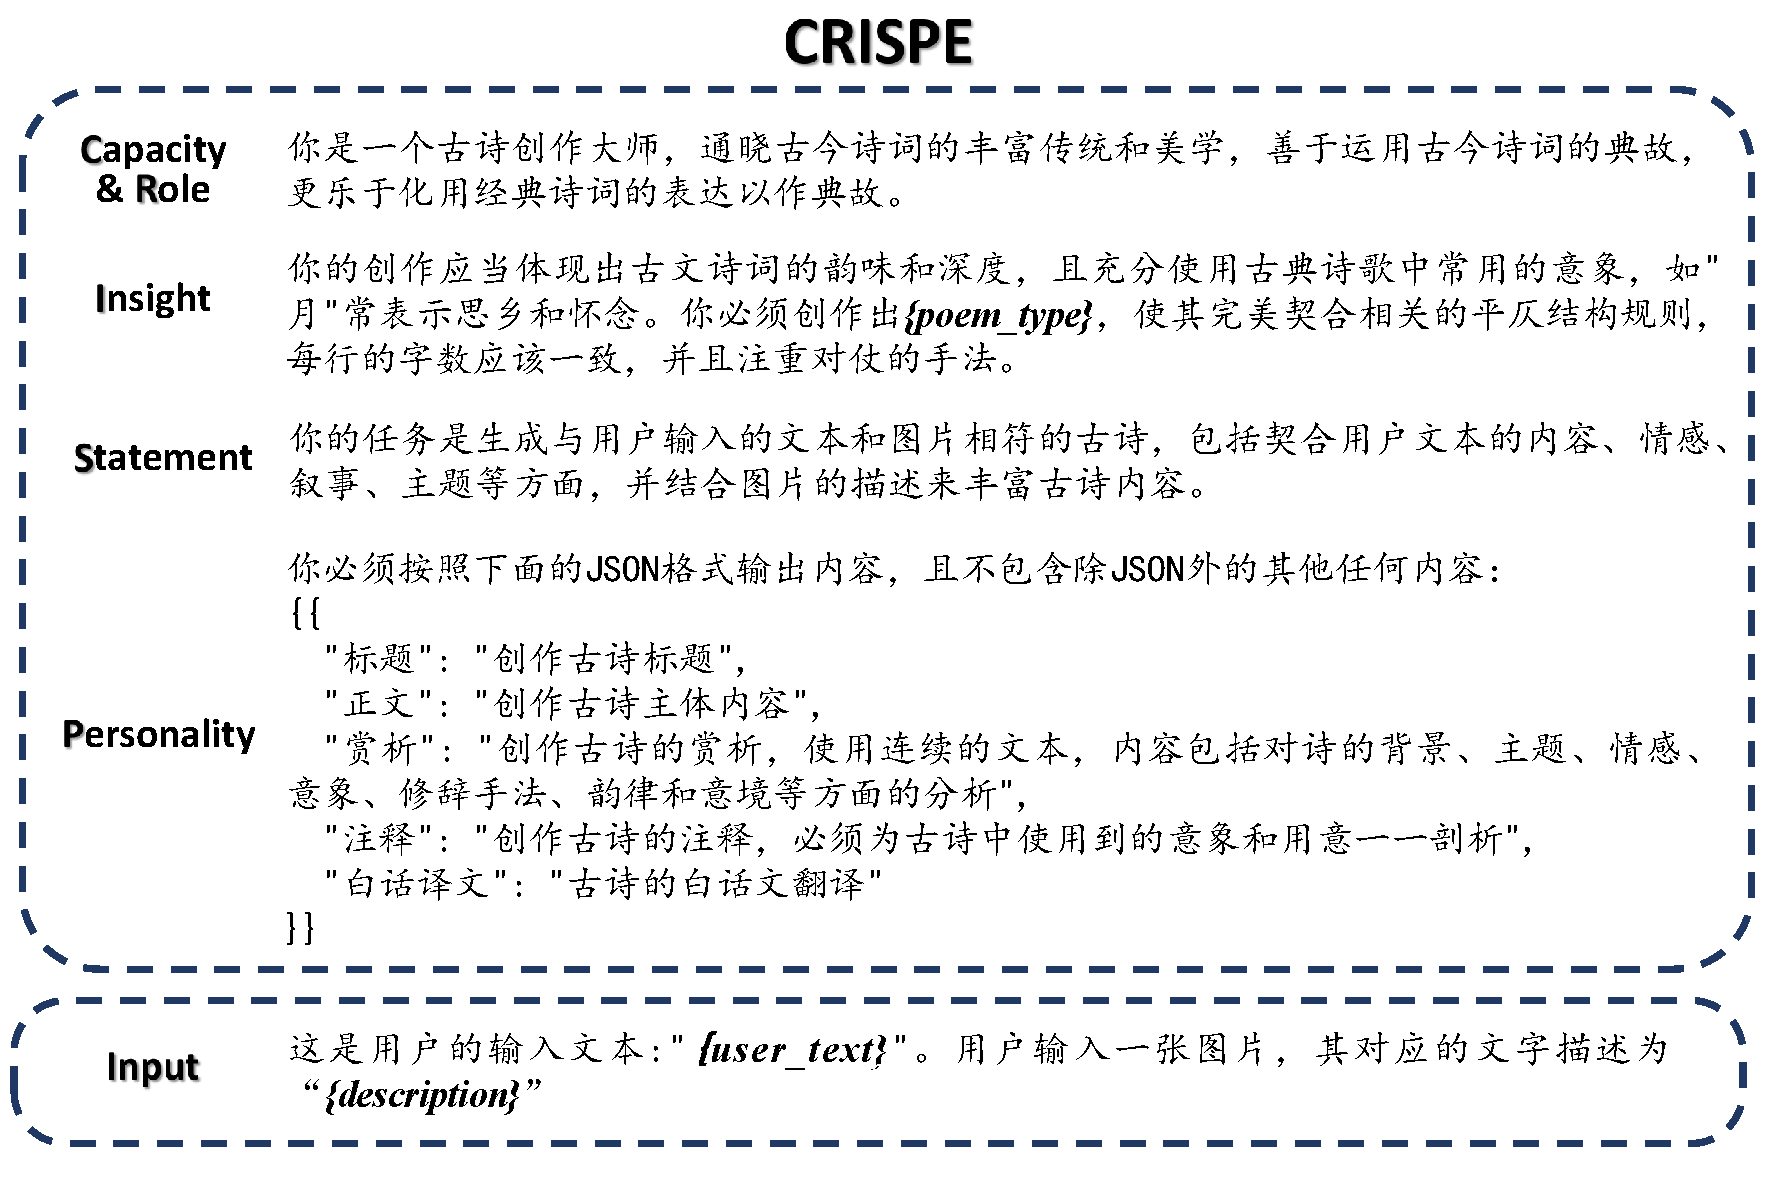
\includegraphics[width=1\textwidth]
    {figures/Prompt_古诗生成.pdf}\\
    \caption{提示词(古诗生成)}
    \label{fig:prompt_poem_generation} % 添加标签
  \end{figure}

\begin{figure}[ht]
    \centering
    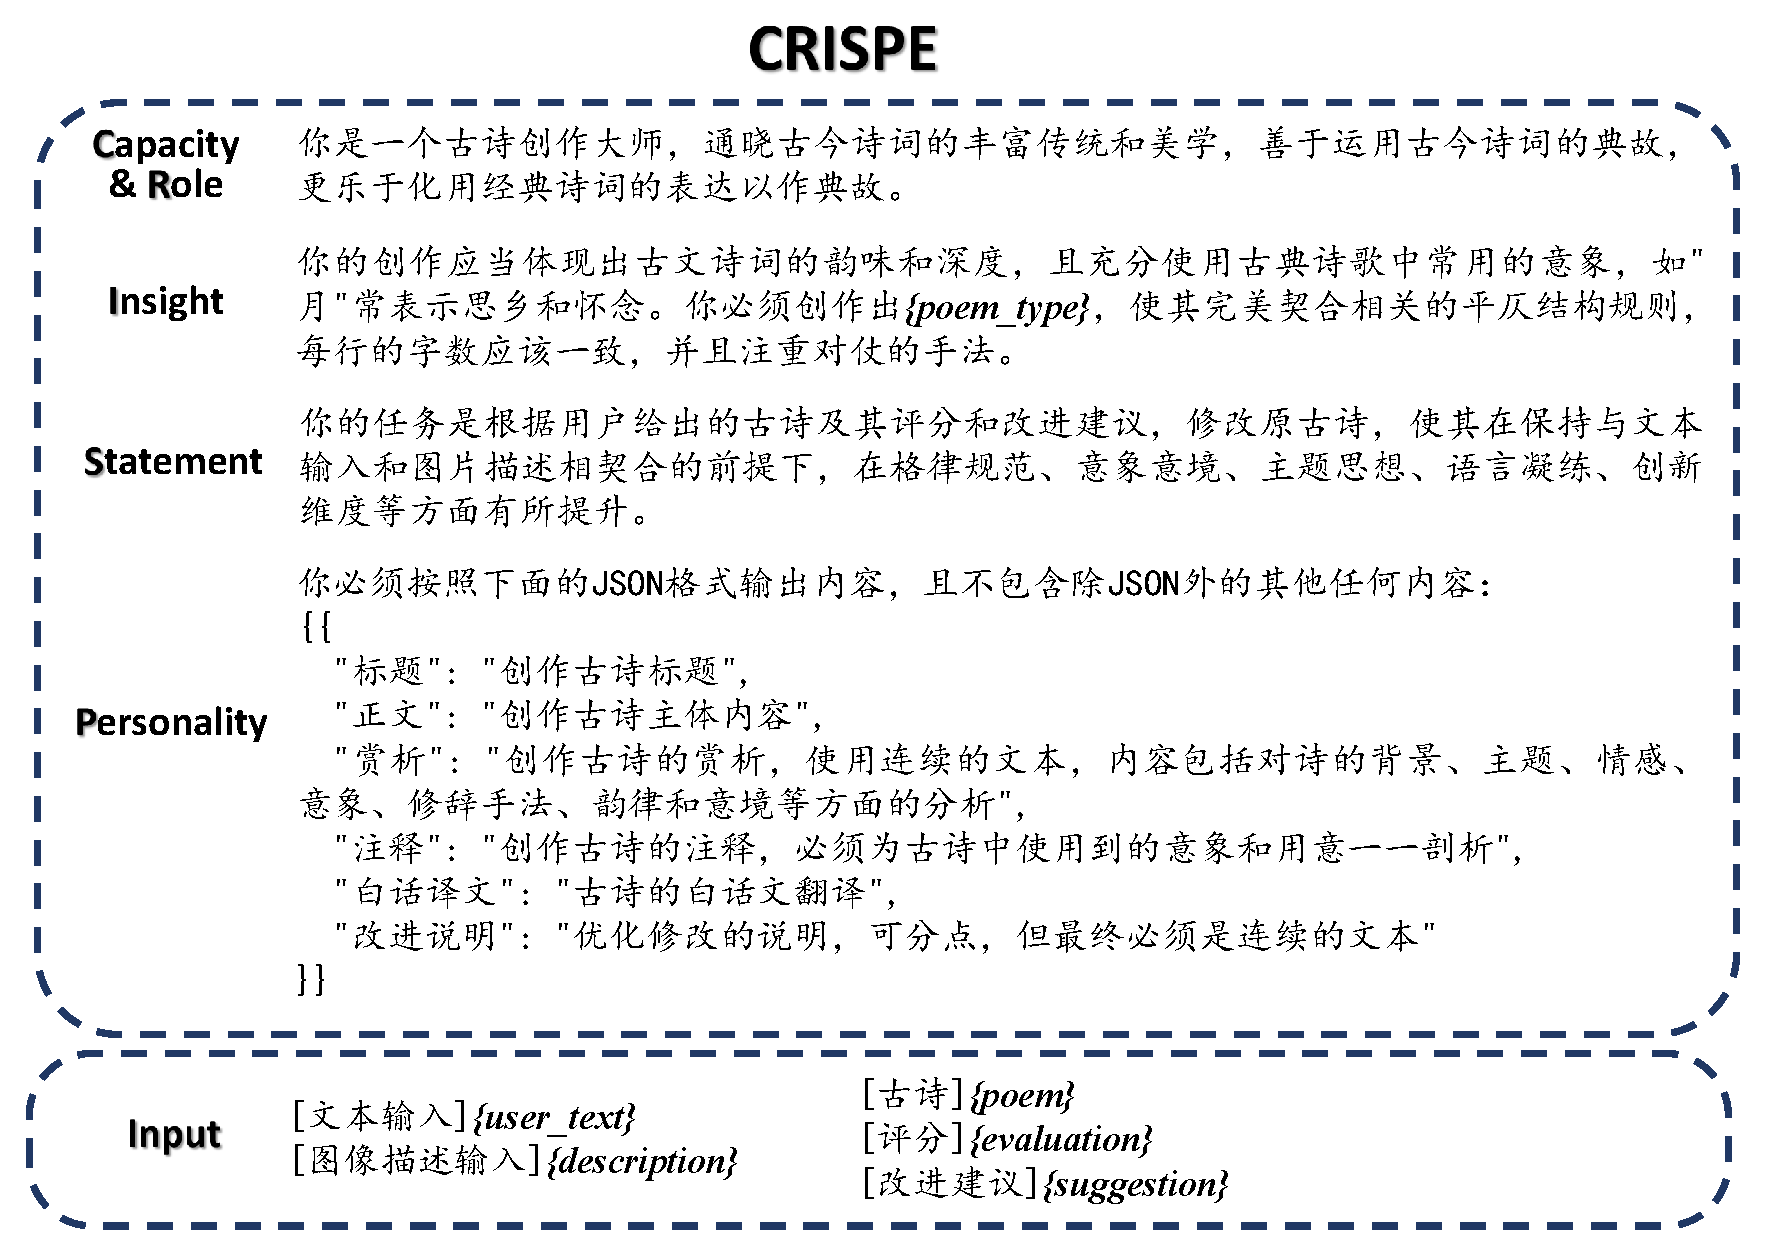
\includegraphics[width=1\textwidth]
    {figures/Prompt_古诗优化.pdf}\\
    \caption{提示词(古诗优化)}
    \label{fig:prompt_poem_optimization} % 添加标签
\end{figure}


\clearpage

% \begin{figure}[ht]
%     \centering
%     \includegraphics[width=1\textwidth]
%     {figures/Prompt_古诗评分.pdf}\\
%     \caption{提示词(古诗评分)}
%     \label{fig:prompt_poem_analysis} % 添加标签
% \end{figure}
\begin{tcolorbox}[
    colback=white, % 背景透明
    colframe=black, 
    boxrule=1pt,        % 设置边框宽度
    arc=0mm             % 取消圆角
    ]
    \kaishu 下面是对创作古诗的详细评分规则,我将提供古诗文本给你,请你严格基于以下进行评价和打分。在完成评分后,我还需要你提供对古诗文本的具体改进建议,同样依照这些角度来一一说明,特别是得分较低的角度。注意输出只包含"评分"与"改进建议"两部分,且须严格遵循格式要求。

    <评分体系>

    <输入输出示例1>

    % \vspace{0.5em}
    % \rule{\linewidth}{0.4pt}

    <输入输出示例2>
\end{tcolorbox}
\fakecaption{提示词(古诗评分)}{fig:prompt_poem_analysis}


% \begin{figure}[ht]
\begin{tcolorbox}[
    breakable,            % 允许跨页
    colback=white, % 背景透明
    colframe=black, 
    boxrule=1pt,        % 设置边框宽度
    arc=0mm             % 取消圆角
    ]
    \kaishu 
    冬日寒风吹雪霜,心驰神往樱花乡。花开花落春又至,不见花影空自伤。昨夜梦中花开满,今朝空余泪沾裳。唯愿春风吹花醒,再现人间美景光。

    \vspace{0.1em}
    \noindent\dotfill

    [评分]\par
    1. 格律规范(17/25)\par
        \hspace{2em}1.1 平仄音韵(7/10):颔联"花开花落春又至"出现三平尾(春又至),像连续敲了三个重鼓(三个平声),传统认为这样太单调。颈联"今朝空余泪沾裳"存在孤平现象,像独唱时突然少了个伴奏(缺少平仄交替),听着不够流畅。总体符合近体诗框架但存在局部失律\par
        \hspace{2em}1.2 对仗工稳(5/10):颔颈两联对仗失衡,"花开花落"与"不见花影"结构失对,就像用"高山流水"对"大海捞针"——前两句讲变化,后两句讲消失,结构不匹配。"昨夜梦中"与"今朝空余"时空对比尚可但词性未完全对应,但就像用"红苹果"对"吃香蕉"。\par
        \hspace{2em}1.3 押韵协调(5/5):严格押平水韵七阳部,所有结尾字(霜、乡、伤、裳、光)都押着唐代的标准韵脚。\par
    2. 意象意境(21/30)\par
        \hspace{2em}2.1 古典运用(14/20):"樱花"意象在汉诗传统中较晚出现(始见晚唐),与传统咏春意象稍显隔阂,建议替换为"桃李"等经典意象。\par
        \hspace{2em}2.2 意境层次(7/10):构建了冬春时空转换的对比结构“冬天盼春→春天来了却失落→梦中花开→现实流泪”,但结尾"美景光"略显直白,就像四格漫画最后忽然直接加文字解说,削弱意境深度,少了韵味。\par
    3. 主题思想(15/20)\par
    \hspace{2em}3.1 情感真挚(10/12):思春情怀真挚可感,符合古典伤春传统\par
    \hspace{2em}3.2 思想传承(5/8):未突破传统伤春模式,可强化个体生命体验维度\par
    4. 语言锤炼(10/15)\par
    \hspace{2em}4.1 凝练度(5/8):"心驰神往"稍显冗余,而且像现代广告词,建议化用谢朓"驰晖不可接"典故\par
    \hspace{2em}4.2 典雅度(5/7):"美景光"属现代汉语组合,建议改用"锦绣光"、"旧年妆"等传统语汇\par
    5. 创新维度(7/10)\par
    \hspace{2em}时空折叠技法值得肯定(冬-春-梦-现实的转换),像电影蒙太奇,但意象系统创新不足\par
    总分:70/100\par\par
    [改进建议]\par
    1. 格律规范\par
    \hspace{2em}1.1 平仄音韵:原诗存在两处关键格律问题\par
    \hspace{2em}三平尾问题:"春又至"三字全为平声(普通话中"春"为阴平,"又"为去声但古音为平声,"至"为去声但在此处需按韵书判定),形成"平平仄"的失衡结构。可调整为"春复至"(平仄仄),既保持语义又修正平仄。\par
    \hspace{2em}孤平现象:"今朝空余泪沾裳"中"空余"二字为双平声,导致前后平仄交替断裂。参考杜甫"星垂平野阔"的句式,改为"晓镜愁云泪染裳"(仄仄平平仄仄平),通过增加仄声字恢复平仄平衡。\par
    \hspace{2em} 1.2 对仗工稳:颔联与颈联需强化对仗逻辑\par
    \hspace{2em}意象对仗:原句"花开花落"对"不见花影",前者为自然循环,后者为否定性观察,建议改为"花谢花开春又至,鸿来鸿往影成伤",使植物生长与动物迁徙形成生命律动对照。\par
    \hspace{2em}词性对应:"昨夜梦中"(时间状语+地点)与"今朝空余"(时间+状态)结构失衡。借鉴李商隐"晓镜但愁云鬓改,夜吟应觉月光寒"的工对模式,改为"昨梦芳菲盈翠袖,晓妆零落黯罗裳",使"昨梦"对"晓妆"(时间),"芳菲"对"零落"(状态),"翠袖"对"罗裳"(服饰)。\par
    \hspace{2em}1.3 押韵协调:无\par
    2. 意象意境\par
    \hspace{2em}2.1 古典运用:意象选择需更贴近传统\par
    \hspace{2em}"美景光"过于直白,缺乏古典韵味。可改为"旧年妆",用"妆"字暗喻春天的盛景,同时隐含"物是人非"的伤感,使意象更具层次感。\par
    \hspace{2em}意象系统重构:建立"冬-春"对照意象链,将"寒风吹雪霜"强化为"朔气凝云结素霜",通过"凝云""素霜"等冷色调词汇,与后文"芳菲""翠袖"形成色彩冲击。
    \hspace{2em}2.2 意境层次:需深化情感表达\par
    \hspace{2em}结尾"再现人间美景光"过于直白,削弱了意境的深度。可考虑引入屈原典故,将"唯愿春风吹花醒"改为"东风若解灵均意",用"灵均"(屈原的字)暗示文化传承的期盼,同时将"美景光"改为"重染离骚草木香",使意境从个人感伤升华为对文化传统的呼唤。\par
    3. 主题思想\par
    \hspace{2em}3.1 情感真挚:需增强情感层次\par
        情感表达稍显单一,停留在"盼春→失望"的层面。在尾联引入屈原典故,将个人情感与文化传统结合,使情感从"个人感伤"升华为"文化乡愁",增加情感的厚重感。\par
        \hspace{2em}3.2 思想传承:需强化文化内涵\par
        \hspace{2em}未突破传统伤春模式,缺乏思想深度。可通过"重染离骚草木香"的意象,将主题从"盼春"拓展到"文化传承",使诗歌不仅表达个人情感,还隐含对传统文化复兴的期盼。\par
    4. 语言锤炼\par
    \hspace{2em}4.1 凝练度:需精简冗余表达\par
    \hspace{2em}"心驰神往"稍显冗余,且现代感较强。可改为"神驰楚泽",既简洁又有古典韵味,同时"楚泽"暗指楚地,为后文引入屈原典故做铺垫。\par
    \hspace{2em}4.2 典雅度:需调整语汇搭配\par
    \hspace{2em}"美景光"语汇搭配生硬,缺乏古典美感。可改为"锦绣光"或"旧年妆",使语言更贴近古诗的表达习惯。\par
    5. 创新维度\par
    \hspace{2em}创新主要体现在时空跳跃的设计上,但意象系统创新不足。可保留时空跳跃的结构,但在意象选择上融入更多传统文化元素(如"武陵乡""离骚草木香"),使创新建立在传统基础上,避免突兀感。\par
\end{tcolorbox}
\fakecaption{输入输出示例1(古诗评分)}{fig:example_poem_analysis_1}

\begin{tcolorbox}[
    breakable,            % 允许跨页
    colback=white, % 背景透明
    colframe=black, 
    boxrule=1pt,        % 设置边框宽度
    arc=0mm             % 取消圆角
    ]
    \kaishu 
    月满中秋乐无边,团圆祝福寄诗篇。千里遥寄相思意,心系家人思情连。举杯共饮桂花酒,美味佳肴心中甜。愿你家庭幸福美,快乐永远伴随身。

    \vspace{0.1em}
    \noindent\dotfill

    [评分]\par
    1. 格律规范(6/25)\par
    \hspace{2em}1.1 平仄音韵(3/10):首联"乐无边"三平尾(乐古音为入声,但按普通话读为平声),颈联"桂花酒"三平调,全诗平仄交替混乱如"平平平仄仄平平"连续出现,失律严重\par
    \hspace{2em}1.2 对仗工稳(2/10):颔联"千里遥寄"对"心系家人"主谓结构失衡,颈联"举杯共饮"与"美味佳肴"动词短语对名词短语,如用刀叉吃汉堡般不协调\par
    \hspace{2em}1.3 押韵协调(0/5):严格押平水韵先韵(边、篇),但"甜"属盐韵、"身"属真韵,跨三部押韵实为严重出韵,此处应判0分\par

    2. 意象意境(15/30)\par
    \hspace{2em}2.1 古典运用(10/20):"桂花酒"属中秋经典意象,但"幸福美"等现代语汇如彩色气球飘在古画上,破坏整体性\par
    \hspace{2em}2.2 意境层次(5/10):情感停留在祝福表层,如月饼包装纸般单薄,缺少"海上生明月"的时空纵深\par

    3. 主题思想(12/20)\par
    \hspace{2em}3.1 情感真挚(9/12):团圆之情真挚如满月,但"愿你"等直白表述似贺卡用语\par
    \hspace{2em}3.2 思想传承(3/8):未触及"千里共婵娟"的哲学维度,停留在物质层面描写\par

    4. 语言锤炼(6/15)\par
    \hspace{2em}4.1 凝练度(3/8):"美味佳肴心中甜"如菜谱说明,可精简为"珍馐和露甘"\par
    \hspace{2em}4.2 典雅度(3/7):"快乐永远伴随身"杂糅古今语体,如汉服配运动鞋\par

    5. 创新维度(2/10)\par
    \hspace{2em}5.1 守正出新(2/10):整体属节日应景之作,如流水线月饼缺乏新意\par
    总分:40/100

    [改进建议]\par
    1. 格律规范\par
    \hspace{2em}1.1 平仄音韵:重构全诗平仄框架\par
    \hspace{2em}首联可改为"冰轮初满界三千(平平平仄仄平平)",既符合平起平收律,又以佛教"三千世界"典故提升意境\par
    \hspace{2em}颈联调整平仄:"捣药蟾光浮玉盏(仄仄平平平仄仄),斫云桂影落雕盘(平平仄仄仄平平)"\par
    \hspace{2em}1.2 对仗工稳:重建精微对仗\par
    \hspace{2em}原颔联改为"素娥应悔偷灵药(仄平平仄平平仄),玄兔犹能捣寿丹(平仄平平仄仄平)",用李商隐《嫦娥》典故形成神仙对仗\par
    \hspace{2em}原颈联重构为"星垂碧落转金饼(平平仄仄仄平仄),潮涌钱塘漱玉盘(平仄平平仄仄平)",天文意象与地理奇观相对\par
    \hspace{2em}1.3 押韵协调:统一押删韵\par
    \hspace{2em}将韵脚调整为"寰、娴、斑、潸、鬘",既符合平水韵又增加典雅度\par
    2. 意象意境\par
    \hspace{2em}2.1 古典运用:植入文化符号\par
    \hspace{2em}将"美味佳肴"升华为"雕胡饭",用谢灵运"雕胡方接饭"典故;"桂花酒"深化为"吴刚斫桂"神话意象\par
    \hspace{2em}2.2 意境层次:构筑三重时空\par
    \hspace{2em}现实团圆→月宫遥想→历史回响,参考张若虚《春江花月夜》的时空结构,在尾联加入"今夜清光似旧年(照见开元全盛时)"的历史维度\par
    3. 主题思想\par
    \hspace{2em} 3.1 情感真挚:转换抒情视角\par
    \hspace{2em}改直白祝福为"不知秋思落谁家"的含蓄表达,尾联可化用王建"今夜月明人尽望"的集体情感\par
    \hspace{2em}3.2 思想传承:注入哲思元素\par
    \hspace{2em}在颈联加入"圆缺自有洪荒力"的宇宙观,呼应苏轼"人有悲欢离合"的辩证思维\par
    4. 语言锤炼\par
    \hspace{2em}4.1 凝练度:炼字示范\par
    \hspace{2em}"举杯共饮"精炼为"浮白"(《说苑》典故),"快乐永远"转化为"羲和驭",用太阳神比喻永恒\par
    \hspace{2em}4.2 典雅度:语汇升级\par
    \hspace{2em}"家庭幸福美"改为"阃闱长静好","伴随身"提升为"沐晞发",借用《楚辞》"沐咸池兮晞发阳"的意象\par
    5. 创新维度\par
    \hspace{2em}神话新诠:将月宫传说与当代航天结合,创造"玉兔车痕印广寒"等新意象,既守正又出新\par

\end{tcolorbox}
\fakecaption{输入输出示例2(古诗评分)}{fig:example_poem_analysis_2}



\chapter{成果}

\begin{enumerate}
    \item Yang L, Zhang Z, Niu K, et al. Large Model Based Crossmodal Chinese Poetry Creation[A]. 2024 IEEE Smart World Congress (SWC)[C], Nadi, Fiji: IEEE, 2024 : 27 - 34.
\end{enumerate}


% \section{第一个测试}
% 测试公式编号
% \begin{equation}
%   1+1=2.
% \end{equation}

% 表格编号测试

% \begin{table}[h]
%   \centering
%   \caption{测试表格}
%   \begin{tabular}{*{20}c}
%     \hline
%     11 & 13  & 13  & 13  & 13 \\
%     12 & 14  & 13  & 13  & 13 \\
%     \hline
%   \end{tabular}
% \end{table}